\section{Simulation and Digitisation}

\subsection{Detector Simulation}
%editors: F. Cossutti & M. Casarsa & L. Gray

%Event reconstruction studies and the study of some final state observables, such as particle identification, are based on a complete \GEANT simulation of the MTD detector. The sensitive detector simulation is recording the initial time and initial and final positions of energy deposited by crossing particles in LYSO and silicon volumes for BTL and ETL, respectively, integrating them in time intervals of 10 ps. 

Gull simulation includes a realistic description of the BTL geometry with crystal bars with their long side orthogonal to the $z$ dimension of the CMS detector. In Fig.~\ref{fig:BTL1} (left) the trays are shown within the Outer Tracker Support Tube, with a radial position of the crystals at 1174.5 mm from the beam axis. The simplified BTL geometry model embedded in the CMSSW framework is based on 48 rows of modules per tray, each including 3 modules of 16$\times$1 crystals of transverse dimensions 57.6 $\times$ 3.15 mm$^2$ with gaps between them corresponding to the space needed by SiPMs. The thickness of the crystals is 3.75, 3 and 2.4~mm, respectively, for each consecutive group of 16 modules moving from the center of the detector towards the endcap region. As shown in Fig.~\ref{fig:BTL1} (right), an aluminum plate with a surface of 92 $\times$ 52.2 mm$^2$ and 3~mm thick is placed below the crystals in front of the tracker volume to simulate the support plate, while a PCB board of equivalent transverse size and 1.6~mm thick is placed 3~mm above the crystals to approximately simulate the readout electronics material budget.

\begin{figure}[hbtp]
\centering
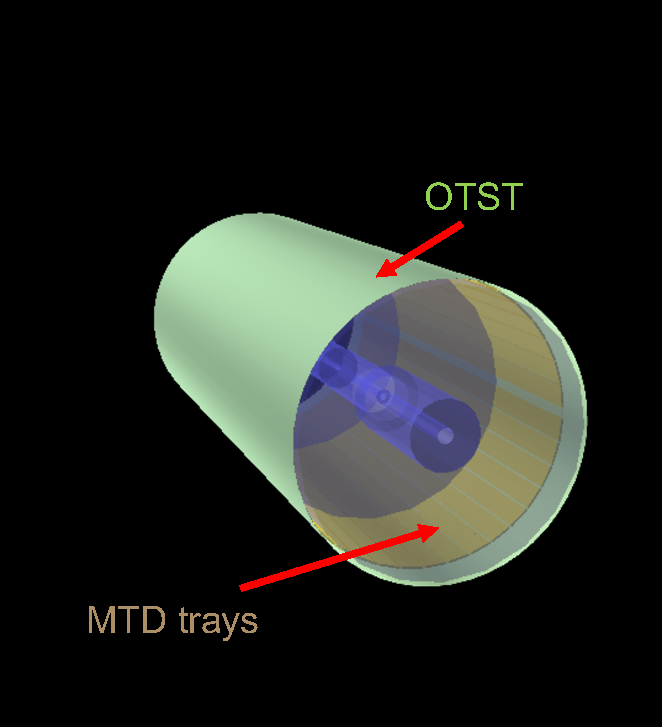
\includegraphics[width=0.49\textwidth]{fig/performance/BTL1.pdf}
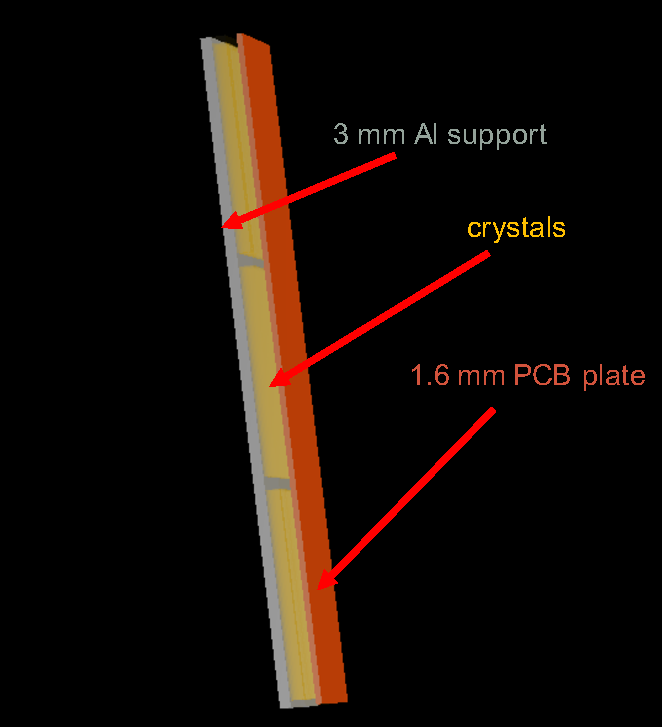
\includegraphics[width=0.49\textwidth]{fig/performance/BTL2.pdf}
\caption{View of the simulated BTL trays within the Outer Tracker Support Tube structure (left) and detailed view of the simulated BTL module (right).}
\label{fig:BTL1}
\end{figure}

%\begin{figure}[hbtp]
%\centering
%\caption{View of the simulated BTL module.}
%\label{fig:BTL2}
%\end{figure}

The ETL description is also included in this full simulation but is representative of the geometry described in the MTD Technical Proposal~\cite{Collaboration:2296612}, because of a limitation in the layout software used to build the MTD geometry in \GEANT.
Since either ETL geometry comprises a hermetic double-layer of silicon, the interleaved double-disk design with radially oriented modules from the TP is sufficient to describe the performance of the $x$-$y$ layout design described in this TDR.
Compared to the TP design, as shown in the left panel of Fig.~\ref{fig:ETL1}, 11 rings of modules have been used for this simulation in the radial acceptance 324--1291~mm, distributed on two disks placed in front of \HGC (right panel of Fig.~\ref{fig:ETL1}) at 3038 and 3057~mm respectively from the interaction center. 
The residual difference between the TP and TDR designs lies in the material distribution of the support structures in the ETL.
An approximate description of the support plate is provided by a set of aluminum disks in between the two sensors' disks.
In both designs the total additional material from the ETL is less than 0.2 $X_0$ (radiation length), and the impact of the variations in material is minimal. 

\begin{figure}[hbtp]
\centering
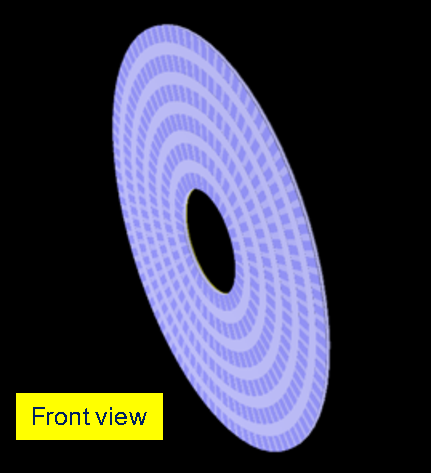
\includegraphics[width=0.49\textwidth]{fig/performance/ETL1.pdf}
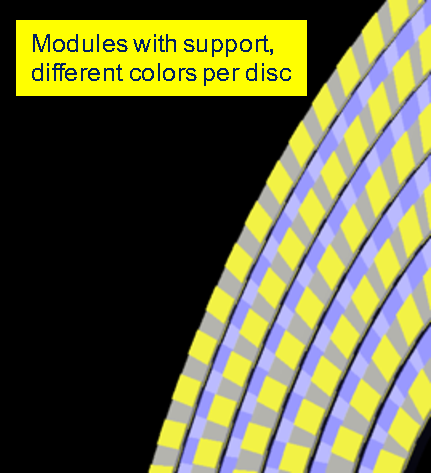
\includegraphics[width=0.49\textwidth]{fig/performance/ETL2.pdf}
\caption{Front view of the simulated ETL structure (left) and detail of the ETL module rings without passive structures, with modules on different disks shown with different colours (right).}
\label{fig:ETL1}
\end{figure}

%\begin{figure}[hbtp]
%\centering
%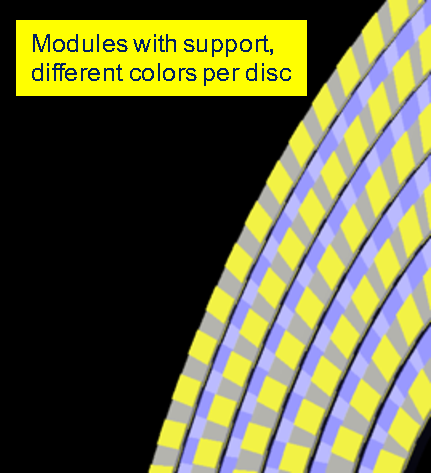
\includegraphics[width=0.55\textwidth]{fig/performance/ETL2.pdf}
%\caption{Detail of the ETL module rings without passive structures, with modules on different disks shown with different colours.}
%\label{fig:ETL2}
%\end{figure}

\subsection{BTL simulation}
\label{sec:btlsim}

The task of the BTL simulation is to convert the energy deposits and
the respective arrival times in a crystal into time and energy
measurements that incorporate the response of the detector
and of the readout chain. 
The total amount of energy deposited in each crystal is estimated via
\GEANT simulation by adding all the energy deposits accumulated in the
crystal within an interval of 25~ns from the bunch crossing. 
The signal amplitudes from the SiPMs at the two ends of the crystal
bar are proportional to the deposited energy through the light yield
(LY) of the crystals and the photon detection efficiency of the SiPMs
(PDE), with a signal sharing depending on the longitudinal position of
the energy position within the crystal bar. 
Table~\ref{tab:sim_parameters} lists the default values for these
parameters, tuned on test beam and laboratory measurements discussed
in Section~\ref{sec:design:BTL:TB_results}.   
The numbers of photoelectrons read out by the ``left'' and ``right'' SiPM are
independently fluctuated according to a Poisson distribution. 

The simulation of the detected time of arrival (TOA) at a given BTL
cell includes different effects: the time of arrival of the first
energy deposit in the cell, a time latency for the scintillation light
to reach to SiPM at the crystal ends, and a time-walk effect depending
on the signal amplitude and the signal discrimination threshold of the
readout electronics. The time latencies from the hit position in the
crystal to the left and right SiPMs are parameterized using
test-beam data, which indicate an average light propagation velocity
of about 8.5~ps/mm in the LYSO bars.  
%
The ability of the BTL readout chip (TOFHIR) to provide two time
measurements per readout channel, either both on the leading edge or
on the leading and trailing edges of the signal, is implemented in the
simulation via a set of configurable parameters. The default
configuration uses the lowest leading edge threshold to digitize the
time of arrival, and a time-walk correction using the amplitude
measurement. 
% 

A reference pulse shape of the TOFHIR signal at the input of the
discriminator is used to
calculate the time-walk delay. The pulse shape is based on a detailed
simulation of the TOFHIR chip based on the CADENCE software.  The pulse
amplitude is normalized to the number of photoelectrons 
and the measured time is set by the time when the pulse crosses a
configurable threshold. 

\begin{table}
  \begin{center}  
    \begin{tabular}{ l | c }
      \hline
      Parameter & Default value \\
      \hline
      LYSO light yield                     & 40000 photons/MeV \\
      Light collection efficiency per SiPM & 0.15  \\ 
      SiPM photon detection efficiency     & 0.20  \\
      Light propagation time in LYSO       & 8.5 ps/mm \\
      \hline
      TOFHIR discriminator thresholds      & 20, 50 p.e. \\
      TOFHIR amplitude threshold           & 4 p.e. \\
      TOFHIR electronic noise              & 1 p.e. \\ 
      Number of ADC bits                   & 10 \\
      ADC range                            & 600 pC \\  
      Number of TDC bits                   & 10 \\
      TDC least significant bit            & 20 ps \\
    \hline
    \end{tabular}
    \caption{Parameters used in the BTL simulation: the values have been tuned on test beam and laboratory measurements.
    \label{tab:sim_parameters}}
  \end{center}
\end{table}

Two time measurements are generated for the left and right SiPMs of a
crystal, $t_{L,\,R}$, which are then independently fluctuated with a
Gauss distribution using a global $\sigma$ that includes all the 
contributions to the time resolution summed in quadrature according to
Eq.~\ref{eq:btl_time_res} and Eq.~\ref{eq:sigma_phot}. 
Finally, the charge and time values are converted into integer numbers according to the TOFHIR specifications 
a 10-bit ADC with a dynamic range of 600 pC (corresponding to 15.6 MeV) and a 10-bit TDC with a granularity of 20~ps
(time saturation at 20.46 ns).

The occupancy is shown in Fig.~\ref{fig:channel_occupancy} (Section~\ref{BTLSec:Electronics}), the BTL crystal occupancy at 200 pileup events, estimated from this simulation, ranges between 6 and 8\%, for signals of amplitude higher than $E_{\text{thr}} = 1$~MeV (about 25\% of the MIP most probable energy deposition), corresponding to the BTL readout threshold. 
At lower thresholds, the occupancy increases --- about 24\% for a threshold of 100~keV --- because of low energy hits, mostly due to out-of-time interactions originating from back-scattered particles from the ECAL. 
According to simulation, these hits are sufficiently delayed with respect to direct tracks to not pile up on the rising edge of the signal, where the time stamp is obtained. 
Furthermore, the average energy deposits from such particles in the LYSO crystals is typically of the order of 5\% of a MIP signal or less. Therefore, their impact on the amplitude measurement used for time-walk corrections is minimal. 
Dedicated simulation studies demonstrated that the impact of both out-of-time pile up and back-scattered particles on the time resolution is below 8 ps.

The acceptance of the BTL has been estimated from the simulation of single muon events and amounts to about 90\%. This efficiency is defined as the probability of finding a cluster of energy deposits (Section~\ref{C5Sec:mtdreco}) larger than 3~MeV spatially associated to a single muon track. 
As shown in the left-panel of Fig.~\ref{fig:BTL_efficiency_pos}, the inefficiency originates from the $\phi$-periodic gaps between adjacent crystal matrices occupied by the SiPMs (two per tray), the gaps between adjacent trays (36 in each half barrel), and the region taken by the tracker support tube rails at $\phi = 0$ and $\phi = \pi$.  
The right panel of Fig.~\ref{fig:BTL_efficiency_pos} shows that hadrons suffer from an additional, $p_{\text{T}}$-dependent inefficiency because of nuclear interactions in the tracker material upstream of the BTL.

\begin{figure}[hbtp]
\centering
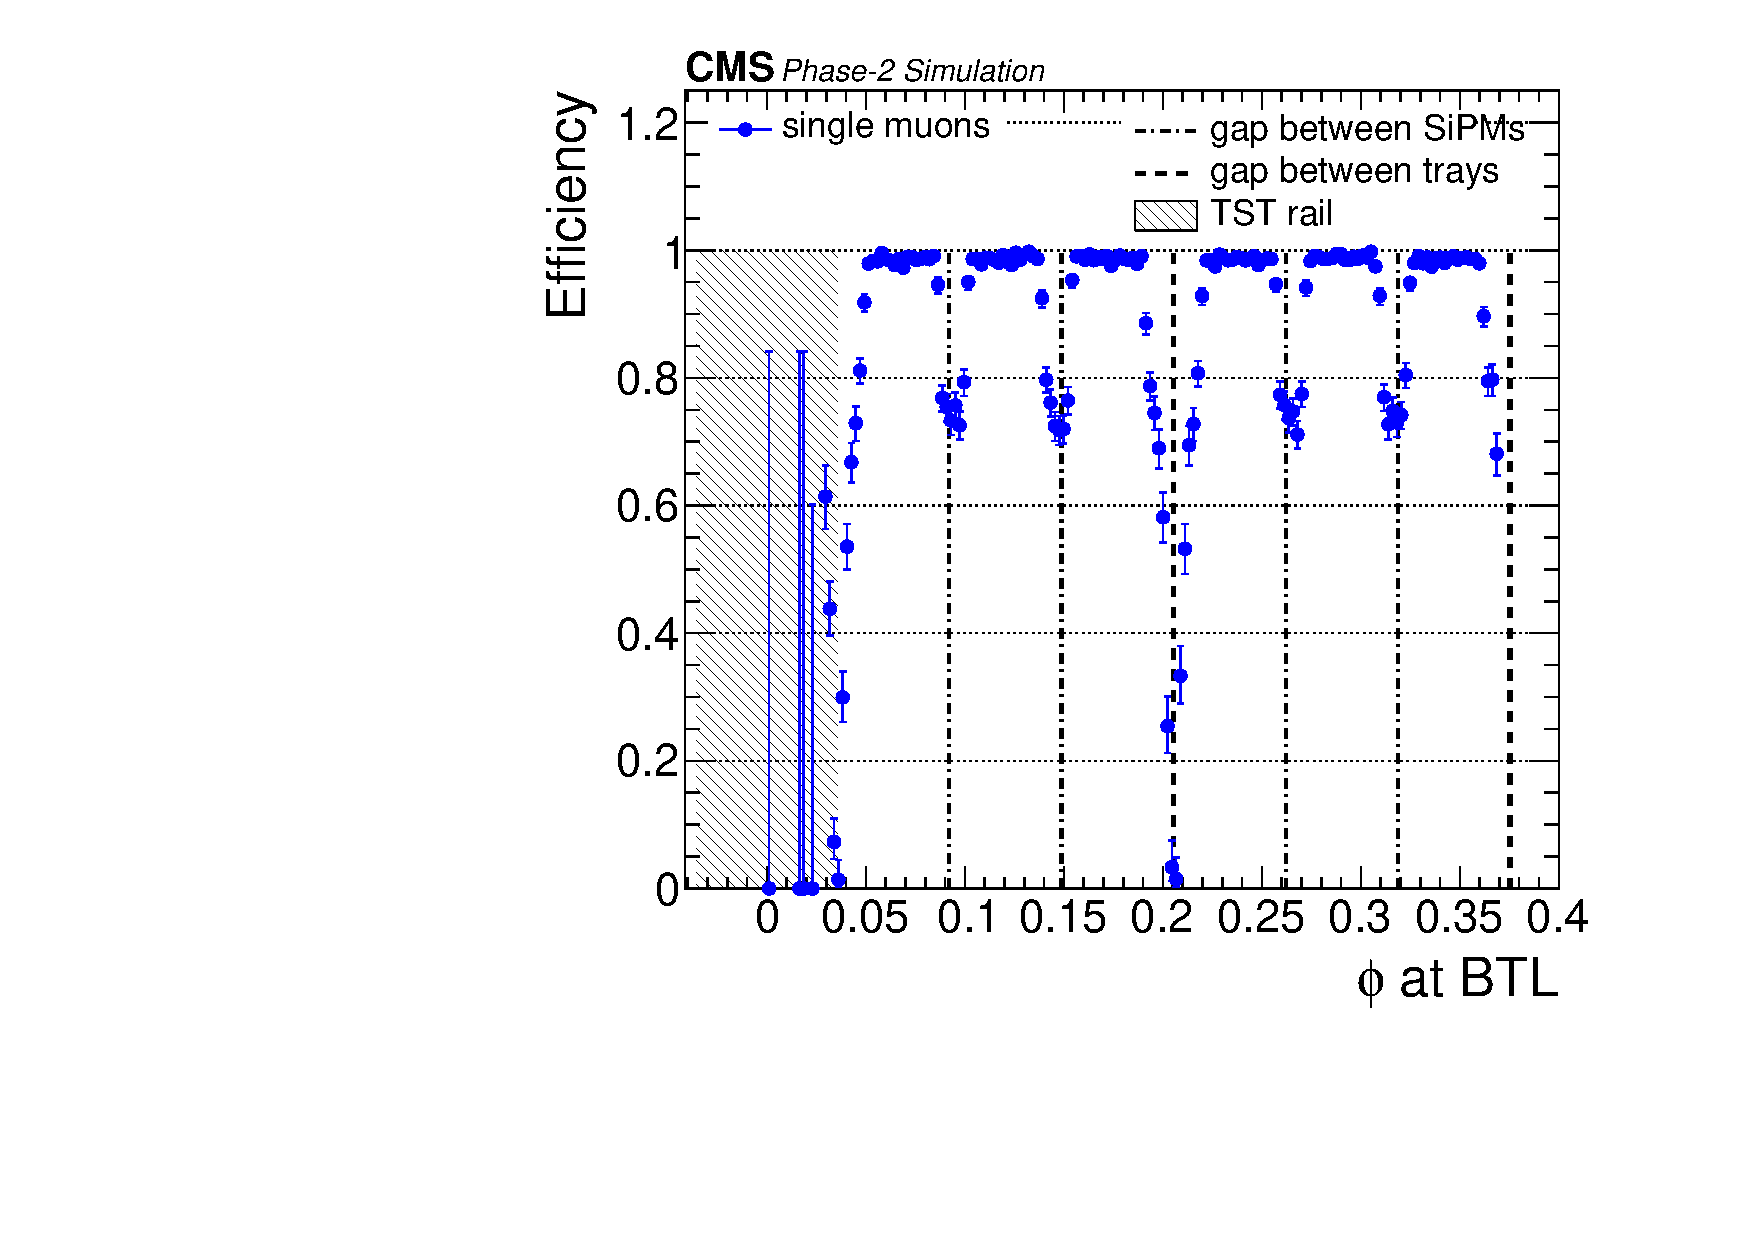
\includegraphics[width=0.49\textwidth]{fig/performance/c_all_efficiency_vs_phi.pdf}
%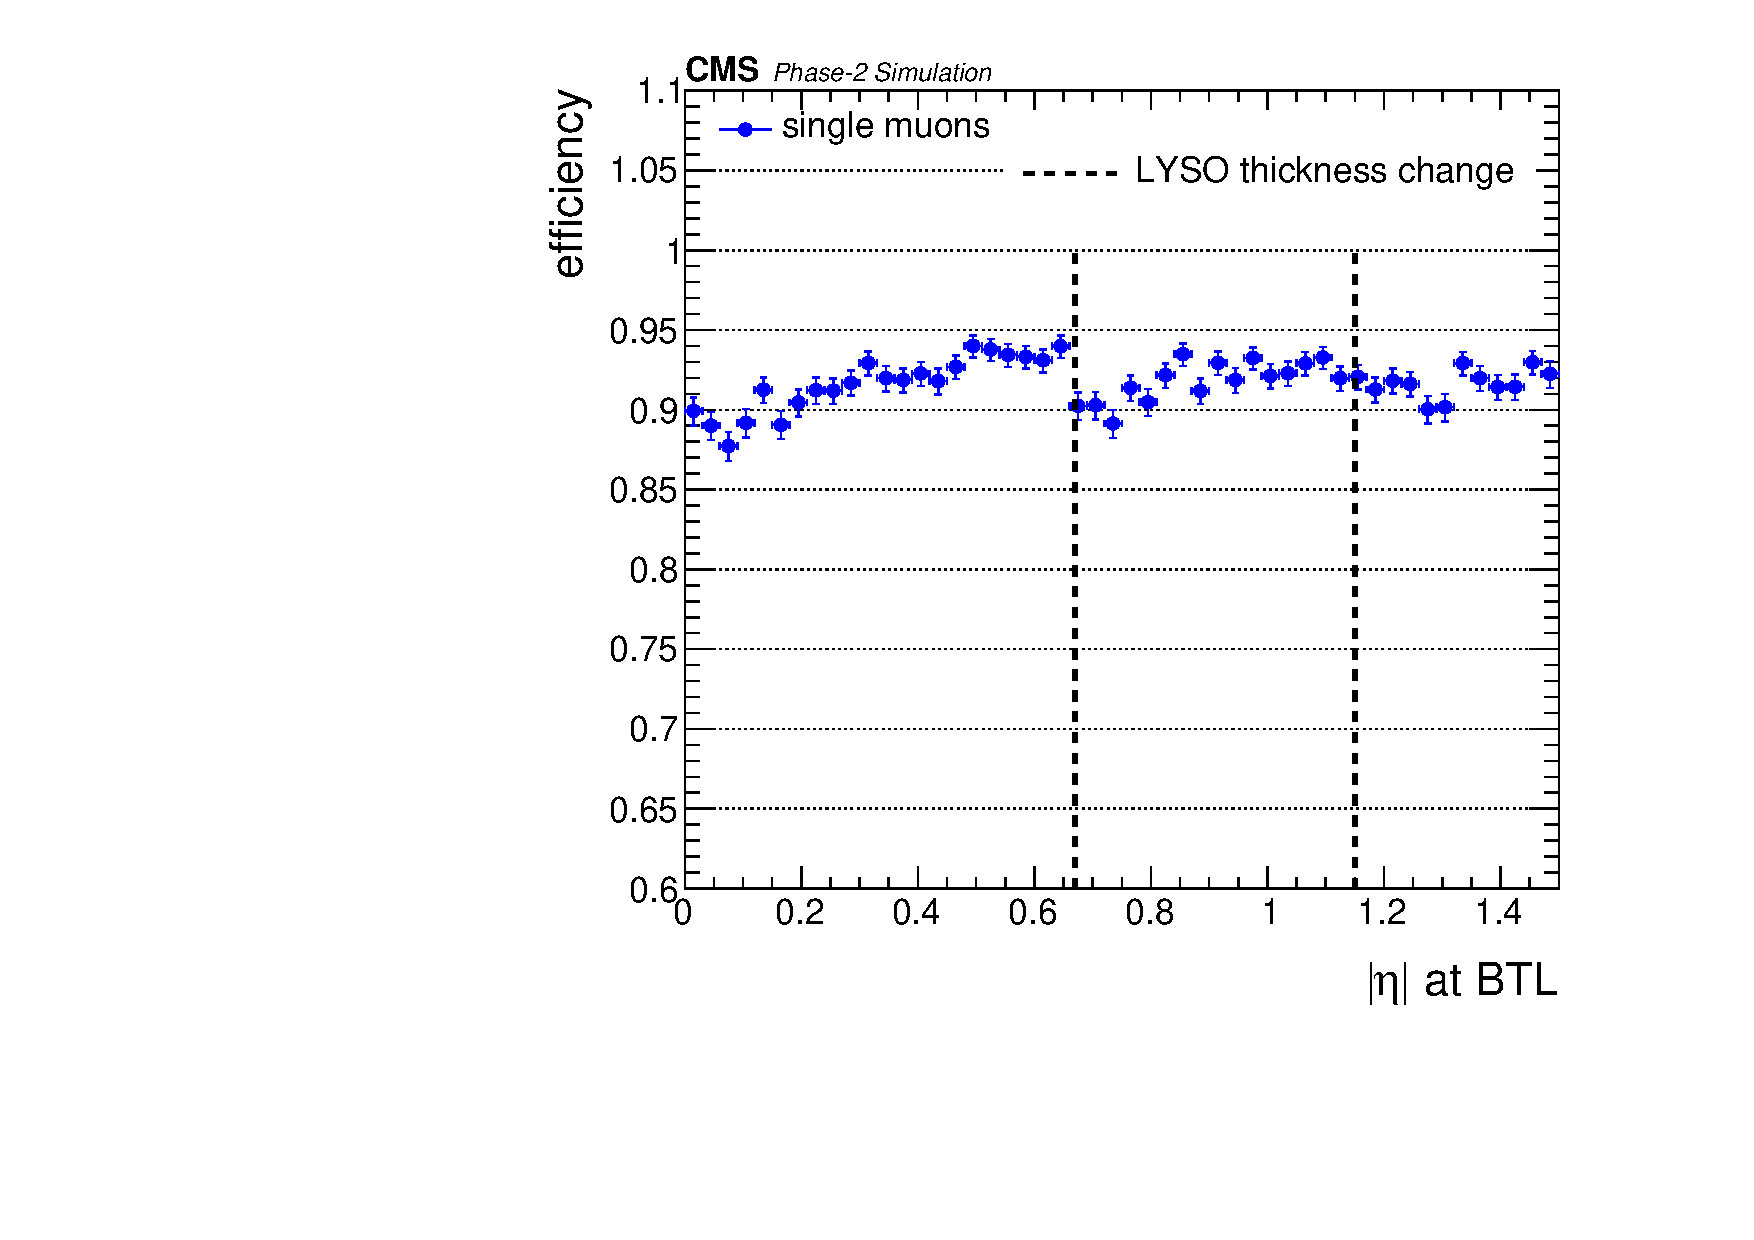
\includegraphics[width=0.48\linewidth]{fig/performance/c_all_efficiency_vs_eta.pdf}
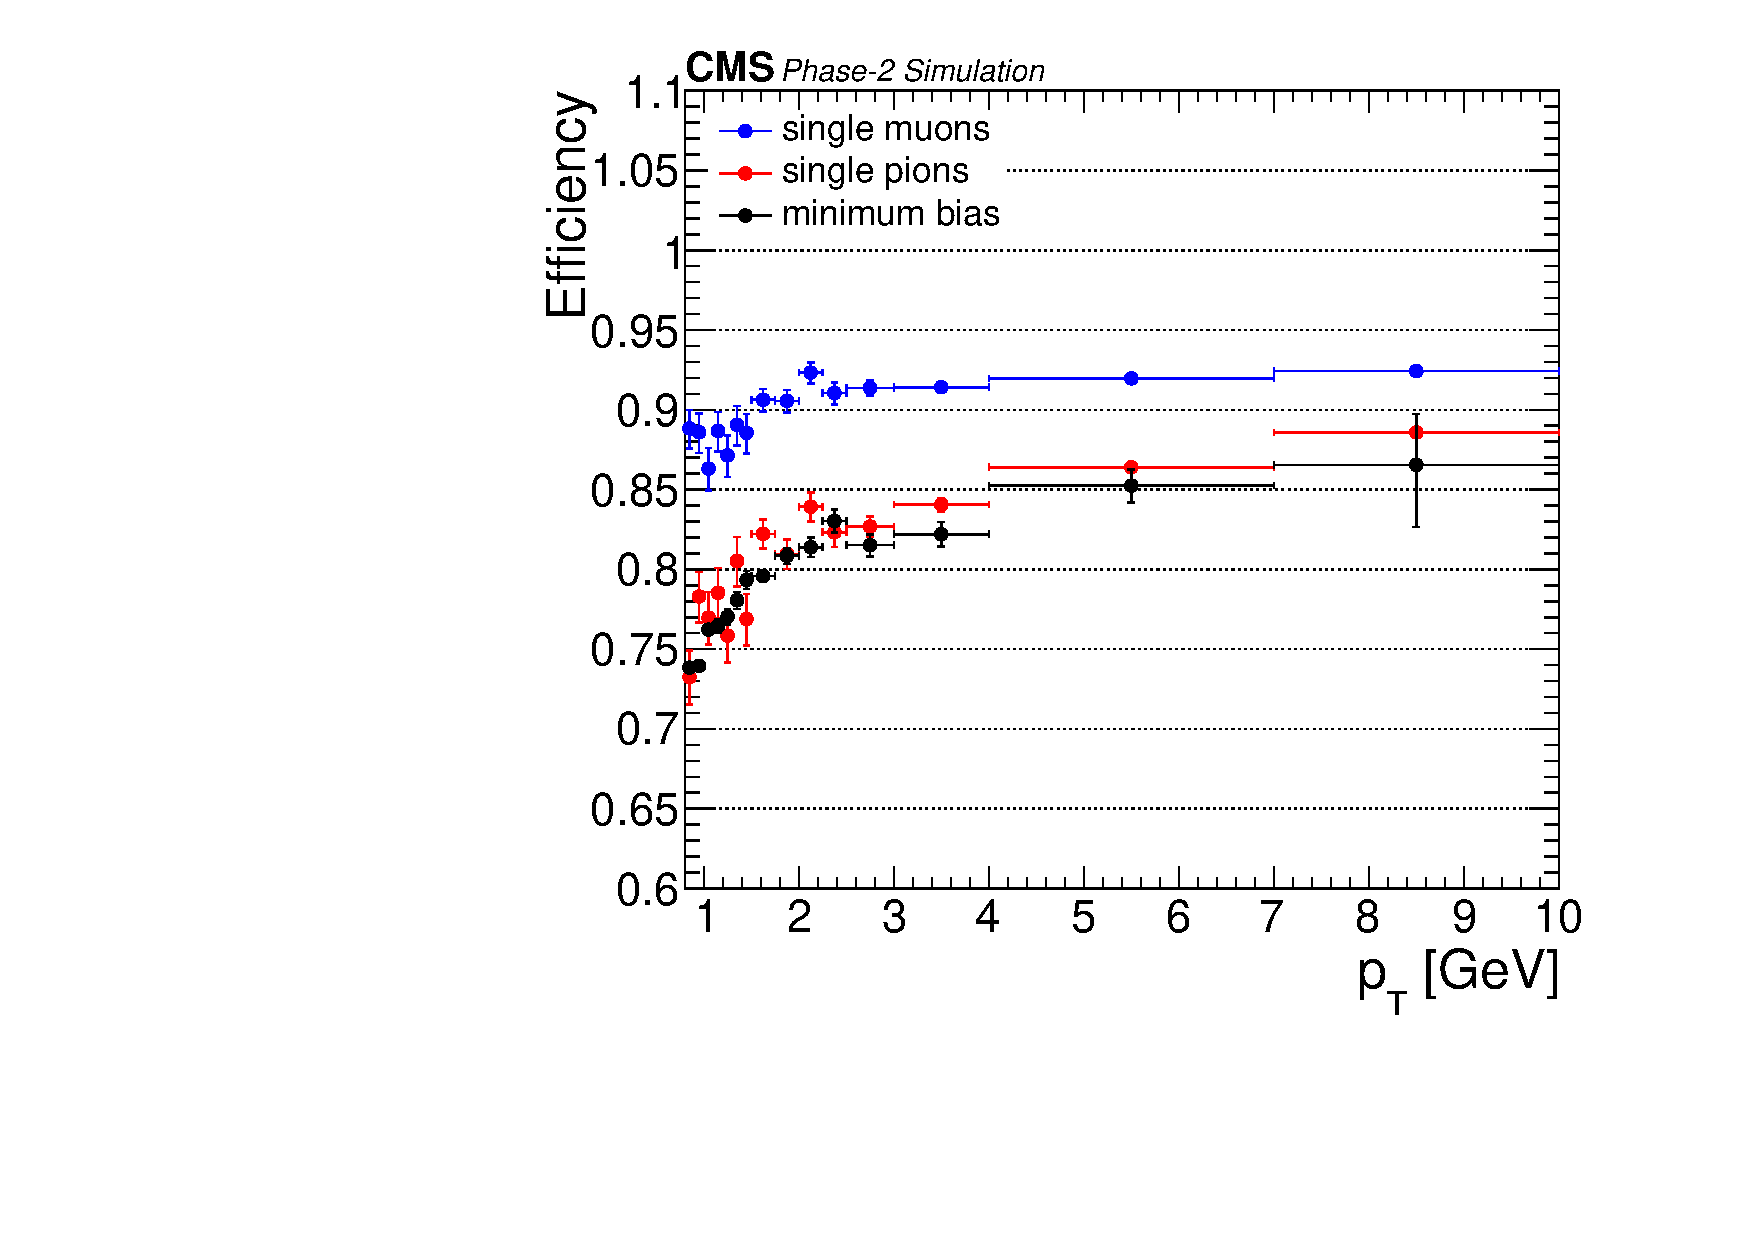
\includegraphics[width=0.49\linewidth]{fig/performance/c_all_efficiency_vs_pt.pdf}
\caption{Per-track efficiency of finding an energy deposit larger than 3 MeV in the BTL and spatially associated to a single muon track. The left panel shows the efficiency as a function of the azimuthal track position at the BTL surface in a range corresponding to two trays. The right panel show the efficiency as a function of the \pt for single muon, single pion, and minimum bias tracks in blue, red, and black, respectively.}
\label{fig:BTL_efficiency_pos}
\end{figure}


\subsection{ETL simulation}
%editors: L. Gray & B. Tannenwald

The ETL simulation follows the description of the geometry given in detail within the MTD Technical Proposal. Eleven overlapping concentric rings of silicon modules are used to develop a detector that is hermetic in $\phi$ for the fiducial region of $1.5 < |\eta| < 3.0$. The full simulation of the ETL layout described in Chapter~\ref{Chapter:ETL}, could not be implemented in time for this document. The timing performance is tuned to
% 15\% comes from 30\% in each endcap and then ETL is half the eta coverage of MTD.
be the two-hit resolution of the ETL described in this document, which will lead to about 15\% of tracks in the fiducial area being covered by the MTD having better performance than the detector described previously in this text, which has a marginal positive impact on higher level physics results. Otherwise, the detectors are acceptance equivalent and so the TP geometry can be used to determine the efficacy of the ETL detector with a high degree of accuracy.

In terms of additional material in front of the CE, both the TP and TDR ETL designs use two layers of aluminium to fix the ETL modules in place, and this drives the material budget of the detector. Hence, the differences in material budget between the TP and TDR ETL versions have minimal impact from the perspective of performance of other detectors. 

%FIXME - Plots (in process).

The per-pad occupancy of the ETL depends on the radial distance to the beam line, but is linear with a moderate slope until the last 5~cm of radius from the support cone. It ranges from 0.1\% at the largest radius to a maximum of 2\% at the smallest radius.
% as demonstrated in Figure~\ref{REPLACE}. NO FIGURE ON ECCUPANCY EXISTS IN THE TDR
Simulated hits are digitized and recorded if their energy is larger than 0.1 MIP-equivalents at normal incidence. The timing resolution of the ETL is currently approximated by using the latest beam test results and the expected performance of the ETROC chip, including the statistical improvement from having two measurements on the track for most tracks. This performance is injected into the simulation of the ETL via a single Gaussian smearing of the crossing time of the accumulated energy at the 0.1~MIP threshold that is also used to trigger the recording of the data. 



%%%PM need to add here similar plot for ETL
%%%Occupancy vs eta with the chosen readout threshold + normal incidence MIP plot
%%%Efficiency of hit finding DR<0.03 vs phi, eta & pt (single mu,single pi and minimum bias

